\chapter{Parametric Phased Array}
%\clearpage
\newpage
\section{Introduction}
Parametric loudspeaker arrays are linear phased transducer arrays, which use the demodulation of ultrasound in air to generate a highly directional and steerable sound source. This effect was first discovered by Westerveld \cite{doi:10.1121/1.1918525} and used in a loudspeaker, the Audio Spotlight, by Masahide Yoneyama and Jun‐ichiroh Fujimoto \cite{doi:10.1121/1.389414}.

Why ultrasound generates a higher directivity is shown in Section \ref{3_sec:directivity}, how the demodulation works in \ref{3_sec:demodulation} and how signal processing tricks can be used to make everything steerable and of better quality is shown in \ref{3_Parametric_array_Sec:Modulation} and \ref{3_Parametric_array_Sec:Array_signal_processing}.
\section{Directivity of ultrasound}\label{3_sec:directivity}
To see, why a linear phased ultrasonic transducer array produces a highly directional beam one needs to know that a transducer can be idealised and modeled as an slit on which a sound wave diffraction's.
To calculate the directivity of a single transducer a model for this transducer has to be introduced. One of the most often used models is the diffraction model, which describes the transducer as a slit on which a incoming planar sound wave is diffracted on. The mathematical foundations for this model are explained in \todo{Preliminaries}. 
The pressure of a transducer in relation to the angle is given as
\begin{equation}
    p(\varphi,r) 
    = 
    \frac{A}{r} \underbrace{\frac{\sin \left ( \frac{ks \sin \phi}{2}\right )}{ \frac{ks \sin \phi}{2}}}_{D_T(\varphi)}
\end{equation}
Where the sinc function is better known as the directivity of the transducer
\begin{equation}
    D_T(\varphi) = \frac{\sin \left ( \frac{ks \sin \phi}{2}\right )}{ \frac{ks \sin \phi}{2}}
\end{equation}
\section{Ultrasonic demodulation in air}\label{3_sec:demodulation}
The most fundamental equation for modeling the non linear behaviour of air is the KZK (Khokhlov, Zabalotskaya and Kuznetsov) equation \cite{MIT_Ultrasound}
\begin{equation}
    \frac{\partial^2 p}{\partial z \partial \tau} 
    = 
    \frac{c_0}{2} \nabla^2_rp
    + 
    \frac{\delta}{2c_0^3}\frac{\partial^3 p}{\partial \tau^3} 
    + 
    \frac{\beta}{2\rho_0c_0^3}\frac{\partial^2 p^2}{\partial \tau^2}.
\end{equation}
Of which the analytical solutions can not be calculated.
However the solution can be approximated by first solving for the linear ultrasonic field $p_1$ by setting the nonlinear term to zero and then solve for the nonlinear solution $p_2$ the final solution is then the superposition of these two fields $p = p_1 + p_2$.
The ultrasonic field $p_1$ is described by 
\begin{equation}
     \frac{\partial^2 p_1}{\partial z \partial \tau} 
    = 
    \frac{c_0}{2} \nabla^2_rp_1 
    + 
    \frac{\delta}{2c_0^3}\frac{\partial^3 p_1}{\partial \tau^3} 
\end{equation}
\textbf{TODO SOLVE}
This solution then can be used as an approximation for the non linear part of the equation
\begin{equation}
     \frac{\partial^2 p_2}{\partial z \partial \tau} 
    = 
    \frac{c_0}{2} \nabla^2_rp_2 
    + 
    \frac{\delta}{2c_0^3}\frac{\partial^3 p_2}{\partial \tau^3} 
    + 
    \frac{\beta}{2\rho_0c_0^3}\frac{\partial^2 p_1^2}{\partial \tau^2}
\end{equation}
which can now be solved near the axis analytically.
The resulting non linear part $p_2$ turns out to be 
\begin{equation}
    p_2 = \frac{\beta P_0^2 a^2}{16 \rho_0 \alpha c_0^4 a^2}\frac{d^2}{dt^2} E^2(t)
\end{equation}
This means that the  pressure of the wave in the farfield is proportional to the second derivative of the squared modulated signal.
\begin{equation}
    p_{FF} \propto \frac{d^2}{dt^2} E^2(t)
\end{equation}
To get now the desired audio signal f(t) as the pressure the envelope needs to be
\begin{equation}
    E(t) = \sqrt{\left ( 1 + m \int \int f(t)dt^2 \right )}.
\end{equation}
But it turns out that this is almost impossible to accomplish because of the bandwidth of the ultrasonic transducers.
Because if the signal $E(t)$ is now modulated onto a carrier signal $f_c$  
\begin{equation}\label{3_Parametric_array_eq:Modulated_Envelope}
    y(t) = E(t) \cos{\left ( 2 \pi f_c \right )}
\end{equation}
the spectrum of the resulting signal $y(t)$ has a very high bandwidth.
\todo{Plot}
Thats why this is not possible and the signal $E(t)$ needs to be approximated different ways to do this are explored in Section \ref{3_Parametric_array_Sec:Modulation}.

\section{Modulation}\label{3_Parametric_array_Sec:Modulation}
\begin{center}
    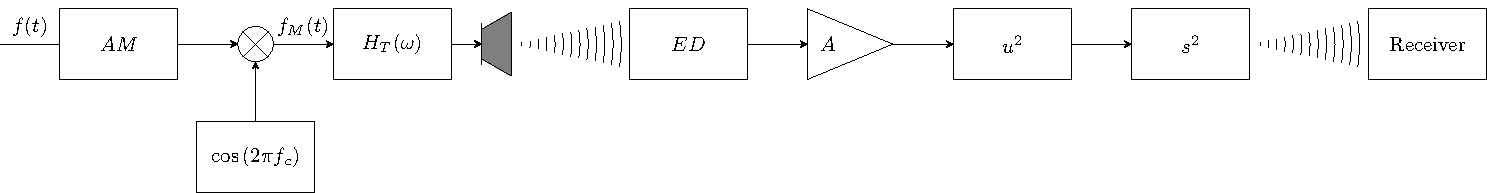
\includegraphics[width=\textwidth]{images/3_Parametric_array/Block_Diagram_Modulation.pdf}
\end{center}
The problem is now that the output signal $u(t)$ of the transducers is not $y(t)$ given in \ref{3_Parametric_array_eq:Modulated_Envelope} but gets influenced by the transfer function of the transducers
\begin{equation}
    U(\omega) = Y(\omega) H_T(\omega)
\end{equation}
The goal now is to make the envelope of the output signal $f_O(t)$ as similar as possible to the square root of the second integral of the input signal
\begin{equation}\label{3_Parametric_array_eq:ideal_signal}
    E \left \{ f_O(t) \right \} = \frac{1}{A}\sqrt{\left ( 1 + m \int \int f(t)dt^2 \right )} = g(t)
\end{equation}
and make it as loud as possible. This optimal signal is defined as $g(t)$
If Equation \ref{3_Parametric_array_eq:ideal_signal} is received at the envelope detector then the original signal is restored at the receiver.
But due to the transfer function of the transducer $H_T(\omega)$ this is not realisable.
The spectrum of the optimal output $f_{TX}(t)$ would need to be
\begin{equation}
    F_{TX}(\omega)
    =
    \frac{1}{A} \mathscr{L}\left ( g(t) \cos{(w_ct)} \right )
    = \frac{A}{2} (G(\omega -\omega_c) + G(\omega +\omega_c)).
\end{equation}
The optimal signal $g(t)$
\begin{equation}
    g(t) = \frac{1}{A}\sqrt{1 + \underbrace{m \int \int f(t)dt^2}_{x(t)}} =  \frac{1}{A}\sqrt{1 + x(t)}
\end{equation}
can be written with a taylor approximation
\begin{equation}
    g(t) 
    = 
    \frac{1}{A} \left ( 1 + \frac{1}{2}x - \frac{1}{8}x^2 + \frac{1}{16}x^3 - \dots \right ) 
    =
    1 - \sum_{k=0}^\infty \frac{2}{k+1} \left ( \binom{2k}{k} \right) \left ( -\frac{x}{4}\right )^{k+1}
\end{equation}
This means that the spectrum $G(\omega)$ of the optimal signal is
\begin{equation}
    G(\omega) = \frac{1}{A} \left ( 1 + \frac{1}{2}X(w) - \frac{1}{8}\left (X(w) * X(w)\right ) \pm \dots \right ).
\end{equation}
This shows that $G(\omega)$ has an infinite bandwidth, because each correlation in frequency, or multiplication in time, doubles the bandwidth.
So an approximation has to be found.
\subsection{AM}
One possible approximation is to use normal amplitude modulation. The transmitted signal $g_{AM}(t)$ would be 
\begin{equation}
    g_{AM}(t) = h_T(t) * (1 + mf(t)).
\end{equation}
Often $H_T(\omega)$ is approximated to be $\frac{1}{s^2}$, which would cancel out the two derivatives
\begin{equation}
    f_{RX}(t) 
    = 
    Ag^2_{AM}(t) 
    =
    A(2mf + m^2f^2(t))
    =
   \underbrace{2Amf(t)}_{\text{Signal}} + \underbrace{2Am^2f^2(t)}_{\text{Distortion term}}.
\end{equation}
If the simplification of $H_T(\omega)$ is not made the spectrum of the received signal becomes
\begin{equation}
    F_{RX}(\omega) = 2A(mF(\omega)H(\omega) + m^2(F(\omega)*F(\omega))H(\omega))
\end{equation}
As one can see the modulation index $m$ is squared inside of the distortion term and only linear in the signal. This means that if the modulation index would be chosen small enough the distortion term would vanish, but the power of the signal would also be reduced significantly. 
\todo{Graphic AM}
\subsection{Modified Amplitude Modulation}
As seen if DSBAM is used there is a problematic distortion term. Modified Amplitude Modulation or MAM uses a similar idea to quadrature amplitude modulation to get rid of this problem \cite{MAM_Main_Paper} .
As the inphase component the input signal $1 + mf(t)$ with a DC offset is used and  as the quadrature component the signal $\sqrt{1 - m^2f^2(t)}$ is used. If now the output signal of the modulation $f_M(t)$ is calculated, as described in \ref{2_QAM_sec:QAM}, it turnes out to be
\begin{equation}
    f_M(t) = \sqrt{2 + 2mf(t)} \sin{\left(\omega_0 t + \arctan{ \left ( \frac{\sqrt{1 - m^2f^2(t)}}{1 + mf(t)} \right )} \right )}.
\end{equation}
If $H_T(\omega)$ is now again assumed to be $H_T(\omega) = \frac{1}{\omega^2}$ the signal turns out to be exactly what is should be. 

This would be a perfect modulation method but again because of the square root in the quadrature component this modulation can not be output by the transducers due to their limited bandwidth. However the basic idea still can be used. This is done by approximating the distortion terms with a taylor series
\begin{equation}
    Q(t) 
    = 
    \sqrt{1 - m^2f^2(t)}
    = 
    \sum_{i=0}^\infty \frac{(2i)!}{(1-2i) i!^2 4^i}m^{2i}g^{2i}(t) 
    \approx 
    \sum_{i=0}^m \frac{(2i)!}{(1-2i) i!^2 4^i}m^{2i}g^{2i}(t).
    \label{3_eq:mam_distortion_approx}
\end{equation}
Depending on the frequency response of the transducers the degree of the approximation $m$ can be chosen. The higher the degree of approximation gets the higher the bandwidth of the transducers have to be.
\todo{Graphic MAM}
\section{Array Signal Processing}\label{3_Parametric_array_Sec:Array_signal_processing}
The theory in this section is mostly taken from the book Fundamentals of Ultrasonic Phased Array \cite{alma99116706330905515}.
\subsection{Phased Array Beam Model}
To explain phenomena such as beamsteering and beamfocusing the multiple slit model isn't meaningful enough and because of that a new model has to be introduced. 
\begin{center}\label{3_Parametric_array_img:Transducer_Model}
    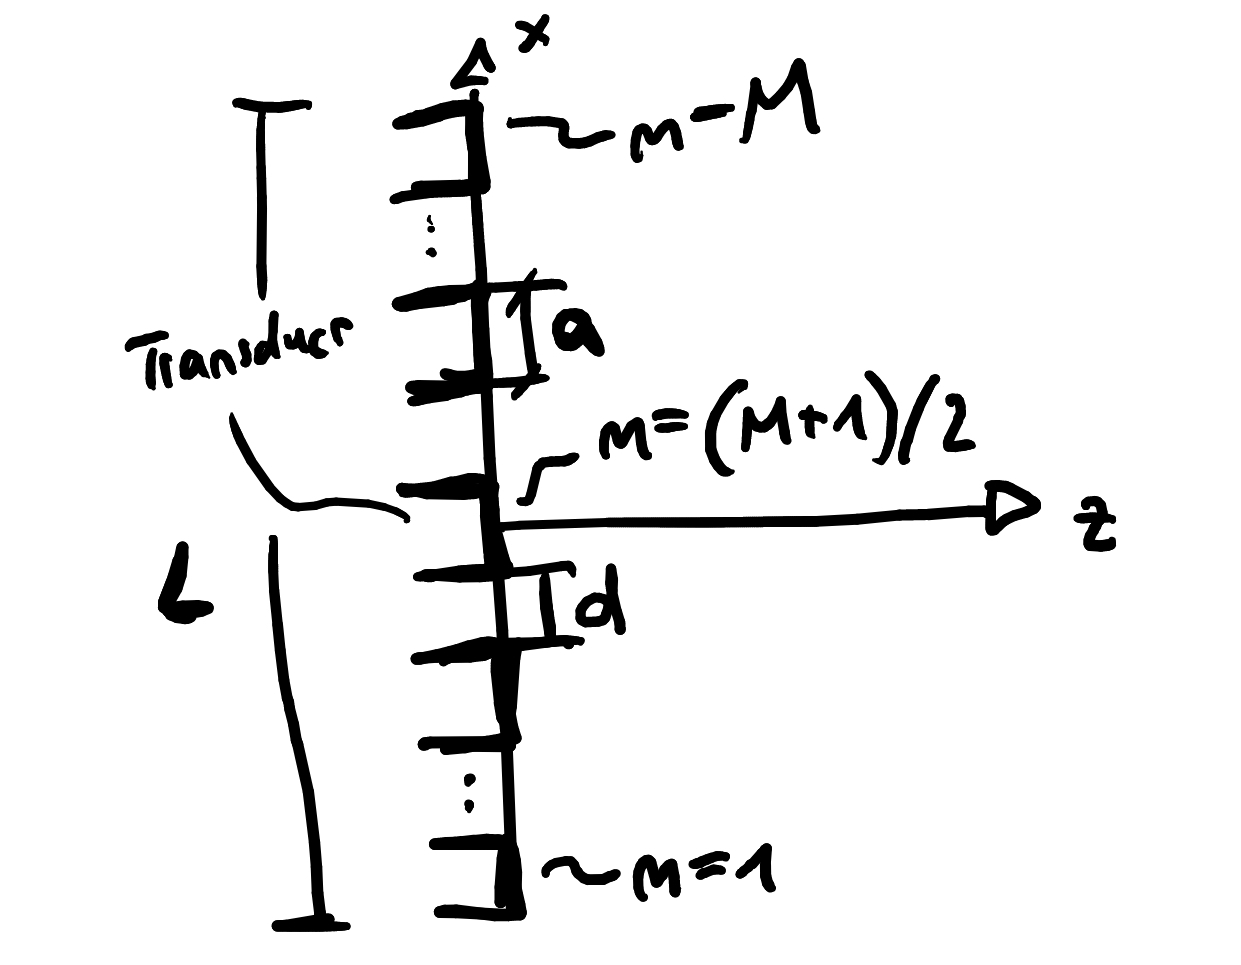
\includegraphics[width=0.3\textwidth]{images/3_Parametric_array/Sketch_TransducerModel.jpg}
\end{center}
Figure \ref{3_Parametric_array_img:Transducer_Model} shows the basic setup of a transducer array with M elements, where M is odd. The position of the mth element is defined as 
\begin{equation}\label{3.4_eq:mposition}
    x_m = -\frac{L}{2} + \frac{a}{2} + (m-1)\cdot(a+d)  
\end{equation}
Where d is the spacing between the transducers, a is the size of the transducers and L is the total length of the array, which is given as 
\begin{equation}\label{3.4_eq:length}
    L = Ma + (M-1)d
\end{equation}
Combining \ref{3.4_eq:mposition} and \ref{3.4_eq:length} gives
\begin{equation}
    x_m = -\frac{Ma + (M-1)d}{2} + \frac{a}{2} + (m-1)\cdot(a+d)  
\end{equation}
Which can be simplified to
\begin{equation}\label{3.4_eq:simplified_xm}
    x_m 
    = 
    \left ( \frac{2m -1 - M}{2} \right ) \underbrace{(d + a)}_{s}
    =
    \left ( \frac{2m -1 - M}{2} \right ) s
\end{equation}
The behaviour of each element can be described as 
\begin{equation}
    p_m(\textbf{x},\omega) 
    =
    \rho c V_0 \frac{k b}{N} \sqrt{\frac{2}{\pi i}} D(\varphi_{m}) \frac{e^{j k b \Bar{r_m}}}{\sqrt{k b \Bar{r_m}}}  
\end{equation}
Where
\begin{equation}
    \Bar{r_m} 
    = 
    \sqrt{\left ( \frac{x}{b} - \frac{e_m}{b}\right )^2 + \left ( \frac{z}{b} \right )^2}
\end{equation}
and 
\begin{equation}
    \varphi_m = \sin^{-1}{\left ( \frac{x - e_m}{b \Bar{r_m}} \right )}
\end{equation}
If now each elements gets its own weighting factor $C_m$ and a phase delay $\Delta t_m$ the pressure at position $\Vec{x}$ of a wave with the frequency $\omega$ can be calulated as 
\begin{equation}
    p(\Vec{x},\omega) 
    = 
    \sum_{i=0}^M C_m e^{j\omega \Delta t_m} \underbrace{\rho c V_0 \frac{k b}{N} \sqrt{\frac{2}{\pi i}} D(\varphi_{m}) \frac{e^{j k b \Bar{r_m}}}{\sqrt{k b \Bar{r_m}}}}_{ p_m(\textbf{x},\omega)} 
\end{equation}
\subsubsection{Far Field}
If only the far field is of interest. Then $\Bar{r}_{m}$ can be simplified to
\begin{equation}
    \Bar{r}_{m} = R - e_m \sin{\varphi}
\end{equation}
and $\varphi_m$ to
\begin{equation}
    \varphi_m = \varphi.
\end{equation}
So the pressure can be approximately written as
\begin{align}
    p(R,\varphi,\omega) 
    &= 
    \sum_{i=0}^M C_m e^{j\omega \Delta t_m} \underbrace{\rho c V_0 \frac{k b}{N} \sqrt{\frac{2}{\pi i}}}_{A} D(\varphi) \underbrace{\frac{e^{j k R}}{\sqrt{k R}}}_{P(R)}e^{-jke_m\sin{(\varphi)}} \\
    &= 
    A D(\varphi) P(R) \sum_{i=0}^M C_m e^{j\omega \Delta t_m} e^{-jke_m\sin{(\varphi)}}
\end{align}
Or with \ref{3.4_eq:simplified_xm} as
\begin{equation}
    p(R,\varphi,\omega) 
    = 
    A D(\varphi) P(R) \sum_{i=0}^M C_m e^{j (\omega \Delta t_m -k \left ( \frac{2m -1 - M}{2} \right )s \sin{(\varphi)} )}
\end{equation}
This is the main model used to explain the directivity pattern of linear phased arrays and with using different weights $C_m$ and delays $t_m$ the behaviour can be explored.

If the weights $C_m = 1$ and $\Delta t_m = 0$ then
\begin{equation}
    p(R,\varphi,\omega) 
    = 
    A D(\varphi) P(R)  e^{jk \left ( \frac{M + 1}{2} \right )s \sin{(\varphi)}} \sum_{m=1}^M \left ( e^{-jks \sin{(\varphi)}} \right ) ^ m
\end{equation}
The last part of the equation above is a geometric series, which can be written as 
\begin{align}
   \sum_{m=1}^M \left ( e^{-jks \sin{(\varphi)}} \right ) ^ m
    &= 
     e^{-jks \sin{(\varphi)}}\frac{1 - e^{-jks \sin{(\varphi) M }}}{1 - e^{-jks \sin{(\varphi)}}} \\
     &=
     e^{-jks\left ( \frac{M + 1}{2}\right ) \sin{(\varphi)}} \frac{\sin{\frac{Mks\sin{(\phi)}}{2}}}{\sin{\frac{ks\sin{(\varphi)}}{2}}}
\end{align}
So the pressure in the far field in relation to $R$,$\phi$ and $\omega$ can be modeled as
\begin{equation}
     p(R,\varphi,\omega) 
    = 
    A D(\varphi) P(R) \frac{\sin{\frac{Mks\sin{(\phi)}}{2}}}{\sin{\frac{ks\sin{(\varphi)}}{2}}}
\end{equation}
\subsection{Array Beamsteering}
If the delays are chosen as
\begin{equation}
    \Delta t_m = \frac{s \sin{\theta}}{c} \left ( (m-1) - \frac{M-1}{2}\right ),
\end{equation}
where $\theta$ is the angle to steer to,
the pressure in the far field is given as
\begin{equation}
     p(R,\varphi,\omega) 
    = 
    A D(\varphi) P(R) \frac{\sin{\frac{Mks(\sin{(\phi)} - \sin{(\theta)})}{2}}}{\sin{\frac{ks(\sin{(\varphi)} - \sin{(\theta)})}{2}}}
\end{equation}
The derivation of this is shown in Appendix ...\todo{Appendix}

\subsection{Beamfocusing}
To focus the beam at a certain radius $R_0$ the delays have to be chosen as
\begin{equation}
    \Delta t_m = \frac{s^2}{2R_0c}(m-1)(M-m)
\end{equation}
for which the pressure in the far field then turns out to be \todo{Calc Far field}. 
\subsection{Array Amplitude Weighting}
As explained in \ref{2_Acoustics_sec:diffraction_fourier} the diffraction process of a grid can be calculated via the fourier transform. If an array of transducers are used the function f(x) is a rectangular sequence. If this rectangular sequence is now sampled with a sampling width of $d$ then the signal is a rectangular window known from FIR filters. The main difference is now that the time axis was replaced by a spatial axis. As in the time domain the nyquist theorem holds and the spatial nyquist frequency is $f = \frac{1}{d}$.
If now weights are applied to the different channels the rectangular window can be changed to other known windowing function and the same theories will hold. 
\subsubsection{Dolph-Chebyshev Window}
The Dolph-Chebyshev Window is a special window used for keeping the size of the side lobes constant. It has one parameter which controls the width of the main lobe and the height of the side lobes. The higher the side lobes are the smaller the main lobe can get. 
\todo{How to calculate}




